So far, we have built a model considering operation time and setup times to for each machine. Doing that, we made an assumption that for any $i$ we would choose the batch production size of product $i$ following the rule $b_i = b_fn_{if}$. We saw that (1) this is not mandatory (but simpler from the point of view of calculations) and that (2) it is not always feasible. In this chapter, we will discuss the case when $b_i \ne b_fn_{if}$. In the first chapter of this part, we established the following formula : 
\[ X_f^{max}(\underline b) = \min_i\left( \frac{\mu_i}{n_{n_{if}}}\right) = \min_i\left( \frac{b_i}{T_{si} + T_{oi}b_i} \middle/ n_{if} \right) \] If we want to produce at a minimum production rate $X_f^*$ we can now compute the minimum batch size on machine $i$ like so \[
    \begin{split}
        X_f^{max}(\underline b) \ge X_f^*
            &\Leftrightarrow \frac{b_i}{T_{si}+T_{oi}b_i}\ge X_f^*n_{if},\forall i\\
            &\Leftrightarrow b_i\ge X_f^*n_{if}T_{si} + X_f^*n_{if}T_{oi}b_i,\forall i\\
            &\Leftrightarrow b_i\ge \frac{X_f^*n_{if}T_{si}}{1 - X_f^*n_{if}T_{oi}}, \forall i
    \end{split}
\]
Futhermore, we know that the production rate for machine $i$ can be computed as $X_i^*=X_f^*n_{if}$ and that the "production" cycle is given by $D_i^*=\frac{b_i}{X_i^*}$. However, how can we draw a GANTT diagram of such a production plan ?

\section{The Kanban organisation}

In this section, we will try to compute the overall "production cycle". That is, from which point in time can we repeat the production of a batch of size $b_i$ for machine $i$. Since every machine can now choose an arbitrary batch size, how can we plan our production ? Well, for it to be repeatable, the overall production cycle $D$ has to be a multiple of each particular machine production cycle $D_i^*$. The minimum one being the \emph{minimum common multiple} of each $D_i$ of the machines. Thus, we have a lower bound for the production cycle which is \[ D^* = \underset{i}{\textrm{mcm}}(D_i^*) \]Note that the \emph{minimum common multiple} doesn't have to be an integer, for example : $\textrm{mcm}\left( \frac{1}{2} ; \frac{1}{4} \right) = \frac{1}{2}$. 

Given these numbers, we can easily input how many items of product $i$ are produced during a whole period $D^*$ since $D^*/D_i^*$ (which is integer) equals the number of batches produced in the time period $D^*$, we get that \[ \#items(i) = \left( \frac{D^*}{D_i^*} \right)b_i \] which can be written in a similar way by substituting $D_i^*$ by its expresion in terms of $b_i$, $n_{if}$ and $X_f^*$ as previously introduced : \begin{equation} \#items(i) = \dfrac{D^*}{ \frac{\cancel{b_i}}{X_f^*n_{if}} }\cancel{b_i} = (D^*X_f^*)n_{if} \label{giving_up:eq1} \end{equation} Finally, since $n_{ff} = 1$, it holds that $\#items(f) = D^*X_f^*$, which makes relation (\ref{giving_up:eq1}) somehow analogous to our initial relation $b_i = b_fn_{if}$.

\begin{wrapfigure}[14]{l}{4cm}
    \centering
    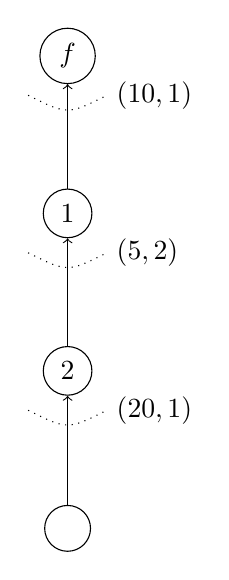
\begin{tikzpicture}
        \draw (0, 0) node[draw, circle] (f) {$f$};
        \draw (0, -2) node[draw, circle] (1) {$1$};
        \draw (0, -4) node[draw, circle] (2) {$2$};
        \draw (0, -6) node[draw, circle] (RM) {$\vphantom{j}$};

        \draw[dotted] (-.5, -.5) .. controls (0, -.75) .. (.5, -.5) node[right] {$(10, 1)$};
        \draw[dotted] (-.5, -2.5) .. controls (0, -2.75) .. (.5, -2.5) node[right] {$(5, 2)$};
        \draw[dotted] (-.5, -4.5) .. controls (0, -4.75) .. (.5, -4.5) node[right] {$(20, 1)$};

        \draw[<-] (f) -- (1);
        \draw[->] (2) -- (1);
        \draw[<-] (2) -- (RM);
    \end{tikzpicture}
    \caption{\label{giving_up:bom1}Example}
\end{wrapfigure}

But let's have an example in order to understand better how we can draw our gantt. Consider figure (\ref{giving_up:bom1}) and a minimum production rate $X_f^* = \frac{1}{3}$. We can easily compute the minimum batch size resulting of that constraint using the previously cited formula like so :
\[
    \begin{split}
        b_f &\ge \frac{\frac{1}{3}.1.10}{1-\frac{1}{3}.1.1} = 5\\
        b_1 &\ge \frac{\frac{1}{3}.1.5}{1 -\frac{1}{3.1.2}} = 5\\
        b_2 &\ge \frac{\frac{1}{3}.1.20}{1-\frac{1}{3}.1.1} = 10
    \end{split}
\]
These lower bounds tell us about the minimum batch size we have to use in order to produce at the minimum rate $X_f^*=\frac{1}{3}$. Thus, we can use greater batch sizes like the following : $b_f = 6$, $b_1 = 5$ and $b_2 = 10$. Using this choice, we can compute each machine's production cycle like so 
\[
    D_f^* = \frac{6}{\frac{1}{3}.1} = 18 = 2.3^2 \textrm{ ; }
    D_1^* = \frac{5}{\frac{1}{3}.1} = 15 = 3.5 \textrm{ ; }
    D_2^* = \frac{10}{\frac{1}{3}} = 30 = 2.3.5
\]
From which we can now deduce the minimum common multiple which is the minimum production cycle for the overall plan : $D^* = 2.3^2.5 = 90$. Assuming these results, you will find in figure (\ref{giving_up:gant1}) the GANTT representation of two production cycles.

\begin{figure}[h!]
    \centering
    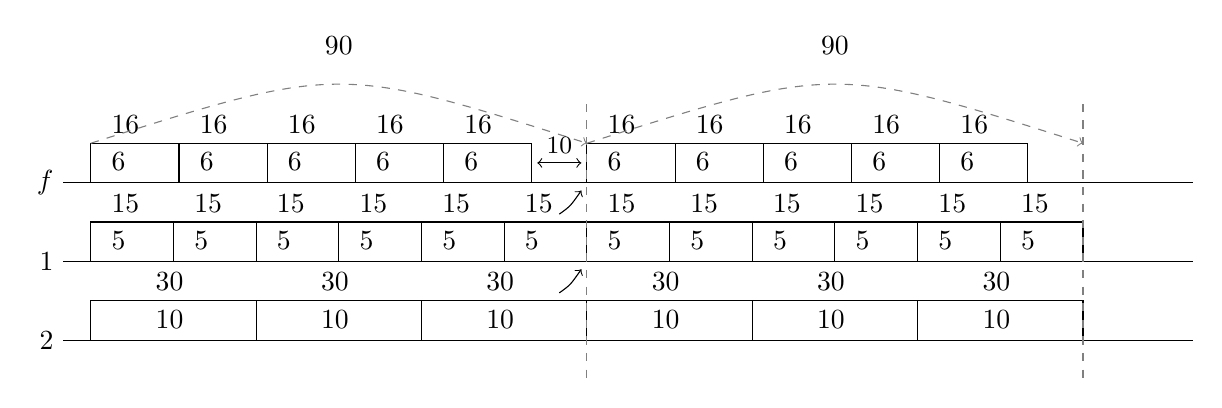
\begin{tikzpicture}[xscale=.07, yscale=.5]
        \draw (-5,0) node[left] {$f$} -- (200, 0);
        \foreach\cycle in {0, 1}
            \foreach \x in {0,...,4} {
                \draw (\cycle * 90 + \x*16, 0) rectangle (\cycle * 90 + \x*16 + 16, 1);
                \draw (\cycle * 90 + \x*16 + 2, 1) node[above right] {$16$};
                \draw (\cycle * 90 + \x*16 + 2, 1) node[below right] {$6$};
            }

        \draw (-5,-2) node[left] {$1$} -- (200, -2);
        \foreach\cycle in {0, 1}
            \foreach \x in {0,...,5} {
                \draw (\cycle * 90 + \x*15, -2) rectangle (\cycle * 90 + \x*15 + 15, -1);
                \draw (\cycle * 90 + \x*15 + 2, -1) node[above right] {$15$};
                \draw (\cycle * 90 + \x*15 + 2, -1) node[below right] {$5$};
            }
        
        \draw (-5,-4) node[left] {$2$} -- (200, -4);
        \foreach\cycle in {0, 1}
            \foreach \x in {0,...,2} {
                \draw (\cycle * 90 + \x*30, -4) rectangle (\cycle * 90 + \x*30 + 30, -3);
                \draw (\cycle * 90 + \x*30 + 10, -3) node[above right] {$30$};
                \draw (\cycle * 90 + \x*30 + 10, -3) node[below right] {$10$};
            }

        \draw[dashed, gray] (90, 2) -- (90, -5);
        \draw[dashed, gray] (180, 2) -- (180, -5);

        \draw[dashed, gray, ->] (0, 1) .. controls (45, 3) .. (90, 1);
        \draw[dashed, gray, ->] (90, 1) .. controls (135, 3) .. (180, 1);
        \draw (45, 3) node[above] {$90$};
        \draw (135, 3) node[above] {$90$};

        \draw[->] (85, -.8) .. controls (87, -.6) .. (89, -.2);
        \draw[->] (85, -2.8) .. controls (87, -2.6) .. (89, -2.2);
        \draw[<->] (81, .5) -- node[above] {\small $10$} (89, .5);
    \end{tikzpicture}
    \caption{\label{giving_up:gant1}Resulting GANTT diagram}
\end{figure}

However, as depicted in figure (\ref{giving_up:gant1}), one may have noticed that we did not fully respect the dependency of product $1$ over product $2$, nor of $f$ over $1$. In fact, it is not possible to draw such a GANTT. To avoid this, we assume the existence of queues in front of each machine and that from now on, the objective for every machine is to fill the queue in front of it when it is emptied. This way of reasonning is called "pull production" since the information flow goes from right to left, whereas in the previous chapters we were referencing to "push production" since it was the raw material which determined when the following tasks could begin. In this view of the production line, every machine starts producing a batch as soon as the queue in front of him is empty. It is called as well KANBAN organisation. 

\section{Using Kanban with $b_i = b_fn_{if}$}

Studying this new kind of systems, we have discovered a new pattern for production scheduling. In this section, we will have a look at what happens if we apply the KANBAN organisation to the situations in which $b_i = b_fn_{if}$. Of course, we have $X_f^* = b_f^*$ which gives us, for machine $i$, a production cycle of \[ D_i^* = \frac{b_fn_{if}}{X_f^*n_{if}} = \frac{b_f}{X_f^*} \] which does not depend on $i$. Computing the overall production rate is trivial since the \emph{minimum common multiple} of a set of identical numbers $D_i^*$ is simply given by $D_i^*$. So that $D^* = D_i^*, \forall i$ since they are the same. 

Using figure (\ref{giving_up:bom1}) again with the same production rate ($\frac{1}{3}$), we can compute $b_f^*$ easily like before. This yields $b_f^* = 10$. Let's say we decide to use $b_f = 12$. Then we can compute the production cycle as $D^* = \frac{12}{\frac{1}{3}} = 36$ (and of course $D^* = D_i^*$) and we can draw, as in figure (\ref{giving_up:gant2}), the GANTT diagram of such a plan. 

\begin{figure}[h!]
    \centering
    \begin{tikzpicture}[xscale=.1, yscale=.5]
        \draw (-5,0) node[left] {$f$} -- (110, 0);
        \draw (-5,-2) node[left] {$1$} -- (110, -2);
        \draw (-5,-4) node[left] {$2$} -- (110, -4);

        \foreach \cycle in {0,...,3} \draw[dashed, gray] (\cycle * 36, 2) -- (\cycle * 36, -6);

        \draw (0,0) rectangle (22, 1);
        \draw (36,0) rectangle (58, 1);
        \draw[pattern=north west lines, pattern color=black!30!green] (72,0) rectangle (94, 1);

        \draw (0,-2) rectangle (29, -1);
        \draw[pattern=north west lines, pattern color=black!30!green] (36,-2) rectangle (65, -1);
        \draw (72,-2) rectangle (72 + 29, -1);

        \draw[pattern=north west lines, pattern color=black!30!green] (0,-4) rectangle (29, -3);
        \draw (36,-4) rectangle (36 + 32, -3);
        \draw (72,-4) rectangle (72 + 32, -3);

        \foreach \cycle in {0,...,2} {
            \draw[<->] (\cycle * 36 + .5, -5) -- (\cycle * 36 + 36 - .5, -5);
            \draw (\cycle * 36 + 18, -5) node[below] {$36$};
            
            \draw (\cycle * 36 + 11, 1) node[below] {$12$};
            \draw (\cycle * 36 + 15.5, -1) node[below] {$12$};
            \draw (\cycle * 36 + 16, -3) node[below] {$12$};

            \draw (\cycle * 36 + 11, 1) node[above] {$22$};
            \draw (\cycle * 36 + 15.5, -1) node[above] {$29$};
            \draw (\cycle * 36 + 16, -3) node[above] {$32$};
        }

    \end{tikzpicture}
    \caption{\label{giving_up:gant2}GANTT diagram using batch size $b_f = 12$}
\end{figure}

If we assume to start the production with empty queues in front of each machine, what would be the time needed to produce the first batch ? Well, as represented by the green rectangles in figure (\ref{giving_up:gant2}), we would roughly need to wait as many production cycles as there are levels in the bill of materials (which means, product dependencies). Thus, the following formula 
\[
    \textrm{Production time of the first batch} \approx \textrm{production cycle}\times\textrm{number of levels of BoM}
\]
In our example, this formula gives us $3\times 36 = 108$, when the real result is $94$.